\documentclass[10pt]{article}
\usepackage{../local}


\newcommand{\classcode}{Physics 105}
\newcommand{\classname}{Analytic Mechanics}
\renewcommand{\maketitle}{%
\hrule height4pt
\large{Eric Du \hfill \classcode}
\newline
\large{HW 03} \Large{\hfill \classname \hfill} \large{\today}
\hrule height4pt \vskip .7em
\normalsize
}
\linespread{1.1}
\begin{document}
    \maketitle
    
    \section*{Collaborators}
    I worked with \textbf{Aren Martinian, Andrew Binder} and \textbf{Adarsh Iyer} to complete this assignment. 

    \section*{Problem 1}
    A bob of mass $m$ is suspended by a massless rigid rod of length $l$ that is hinged to a sled of mass $M$. THe sled slides without friction on a horizontal rail, as shown in the figure.

    \begin{center}
        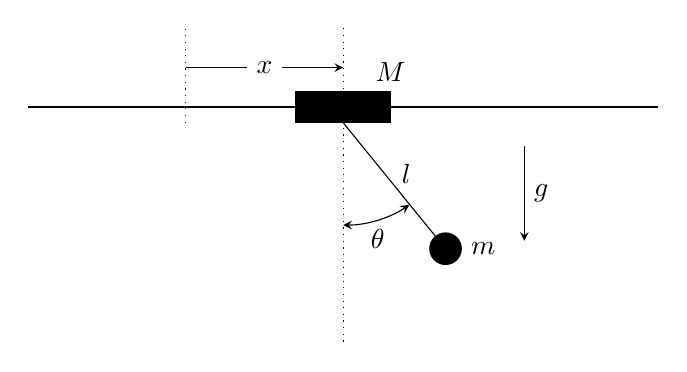
\begin{tikzpicture}
            \draw (-4, 0) -- (4, 0);
            \filldraw[black] (-0.6, -0.2) -- (-0.6, 0.2) -- (0.6, 0.2) node[above] {$M$} -- (0.6, -0.2) -- cycle;
            \draw [dotted] (-2, -0.2) -- (-2, 1);
            \draw [-stealth] (-2, 0.5) -- (0, 0.5) node[midway,fill=white]{$x$};
            \draw [dotted] (0, 1) -- (0, -3);
            \draw (0, -0.2) --(1.3, -1.8);
            \draw (0.8, -1.1) node[above] {$l$};
            \filldraw (1.3, -1.8) circle (0.2cm);
            \draw (1.5, -1.8) node[right] {$m$};
            \draw[-stealth] (2.3, -0.5) -- (2.3, -1.7) node[midway, right] {$g$};
            \draw[stealth-stealth] (0, -1.5) arc(270:304:1.5) node[midway, below] {$\theta$};
        \end{tikzpicture}
    \end{center}
        \begin{enumerate}[label=(\alph*)]
            \item Write down the Lagrangian for the system and derive the equations of motion. 
            
            \begin{solution}
                We can first express the coordinates of the mass bob in cartesian coordinates:
                \[ X = x + l \sin \theta \ Y = -l \cos \theta\]
                so this leads to the equations:
                \[ \dot X = \dot x + l\dot \theta \cos \theta \ \dot Y = l\dot \theta \sin \theta\]
                Therefore, the kinetic energy term is (skipping the intermediate algebra): 
                \begin{align*}
                    T &= \frac 12 M (\dot X^2 + \dot Y^2) + \frac 12 M \dot x^2 \\
                    &= \frac{\dot x^2}{2}(m + M) + \frac{m}{2} \left( 2 \dot x l \dot \theta \cos \theta + l^2 \dot \theta^2\right)
                \end{align*}
                Now, let the sled have zero potential energy. Therefore: 
                \[ U = mgl(1 - \cos \theta)\] 
                And so therefore, the Lagrangian is:
                \[ \mathcal L = T - U = \frac{\dot x^2}{2}(m + M) + \frac{m}{2} \left( 2 \dot x l \dot \theta \cos \theta + l^2 \dot \theta^2\right) - mgl(1 - \cos \theta)\]
                With this now, we recognize that $x$ and $\theta$ are our coordinates, so there are two Euler-Lagrange equations. 
                \begin{align*}
                    \pdv{\mathcal L}{x} - \dv{t}\pdv{\mathcal L}{\dot x} =0 &= -\dv{t}\left( \dot x(m + M) + ml\dot\theta \cos \theta\right)\\
                    0 &= \ddot x(m + M) + ml \ddot \theta \cos \theta - ml \dot \theta^2 \sin \theta
                \end{align*}
                and likewise for the $\theta$ direction:
                \begin{align*}
                    \pdv{\mathcal L}{\theta} - \dv{t}\pdv{\mathcal L}{\dot \theta} = 0 &= -m \dot x l \dot \theta \sin \theta - mgl \dot \theta \sin \theta - \dv{t}\left( m \dot x l \cos \theta - m l^2 \dot \theta\right)\\
                    0 &= ml^2 \ddot \theta + m\ddot x l \cos \theta + mgl \sin \theta
                \end{align*}
            \end{solution}
            \item Suppose, for all $t < 0$, the masses are at rest with $\theta = 0$. Then, at $t = 0$, an impulse $\Delta P = F\Delta t$ is applied to the bob over a small timespan $\Delta t$ from a sharp horizontal tap. Find $\dot x$ and $\dot \theta$ immediately after the tap. (Hint: Consider both linear and angular momentum)
            
            \begin{solution}
                Based on the principles of linear and angular momentum, we know that 
                \[ \Delta p = \pdv{\mathcal L}{\dot x} \phantom{aaaaaaaaa} l \Delta p = \pdv{\mathcal L}{\dot \theta}\]
                And so therefore we get the following system of equations:
                \begin{align*}
                    \Delta p &= \dot x(m + M) + ml \dot \theta \cos \theta, \\
                    l \Delta p &= m\dot x l \cos \theta + m l^2 \dot \theta
                \end{align*}
                Multiplying the top equation by $l$ and subtracting the second, we get:
                \begin{align*}
                    \dot x l(m + M) + ml^2 \dot \theta &= m\dot x l + ml^2 \dot \theta\\
                    Ml \dot x &= 0 \\
                    \therefore \dot x = 0
                \end{align*}
                Then, since $\dot x = 0$, then we also have $\Delta p = ml \dot \theta$ so $\dot \theta = \dfrac{\Delta p}{ml}$.
            \end{solution}
            \item Suppose the impulse $\Delta P$ in (b) is also small, so that the $\theta$ stays small for all $t$. Use the small angle approximation to simplify your equations of motion from (a), and sovle for $x(t)$ and $\theta(t)$ in this approximation.
            
            \begin{solution}
                To simplify our equations of motion, we use the simplificaitons that $\cos \theta \approx 1$ and $\sin \theta \approx \theta$. Doing so, we get the equations: 
                \begin{align*}
                    \ddot x (m + M) + ml \ddot \theta - ml \dot \theta^2 \theta &= 0\\
                    ml^2 \ddot \theta + m \ddot x l + mgl \theta &= 0
                \end{align*}
                From the second equation, we get that $\ddot x = -g\theta - l \ddot \theta$, which we can then plug into the first equation: 
                \begin{align*}
                    (-g\theta - l\ddot \theta)(m + M) + ml\ddot \theta &= 0\\
                    Ml\ddot \theta + g(m+M) = 0\\
                    \therefore \ddot \theta + \frac{g(m+M)}{Ml}\theta = 0
                \end{align*}
                This equation just simple harmonic motion, with $\omega^2 = \frac{g(m+M)}{Ml}$, so we can conclude:
                \[ \theta(t) = A \cos (\omega t) + B\sin(\omega t)\] 
                And since we know that $\theta(0) = 0$, then we choose $\theta(t) = B\sin(\omega t)$ to simplify our calculations. We can solve for $B$ by finding $\dot \theta(0) = \frac{\Delta P}{ml}$, so we get:
                \begin{align*}
                    \dot \theta(0) &= B\omega\cos(\omega t) = \frac{\Delta P}{ml}\\
                    \therefore B &= \frac{\Delta P}{ml\omega}
                \end{align*}
                Now we can proceed to find $x(t)$. To do so, we first need to find $\ddot x(t)$, which requires $\ddot \theta(t)$. So taking two time derivatives, we get:
                \[ \ddot \theta(t) = -\frac{\Delta P}{ml\omega} \omega^2 \sin(\omega t) \] 
                And so now we can plug: 
                \begin{align*}
                    0 &= \ddot x(m+ M) + ml\cdot -\frac{\Delta P}{ml}\omega \sin (\omega t)\\
                    \ddot x &= \frac{\Delta P \omega}{m +M} \sin (\omega t)
                \end{align*}
                which we can now integrate: 
                \[ \dot x = -\frac{\Delta P \omega}{m +M} \frac 1\omega \cos(\omega t) + C_1\] 
                $C_1$ can be determined by using the condition that $\dot x(0) = 0$ from part (b), so therefore: 
                \[ C_1 = \frac{\Delta P}{m+M}\]
                Now we can integrate again to get $x(t)$: 
                \[ x(t) = -\frac{\Delta P}{\omega(m+M)}\sin(\omega t) + \frac{\Delta Pt}{m+M} + C_2\]
                Then we can set $x(0) = x_0$, some arbitrary position, which gives: 
                \[ C_2 = x_0\]
                And so therefore our full equation for $x(t)$ is:
                \[ x(t) = -\frac{\Delta P}{\omega (m+M)}\sin(\omega t)  + \frac{\Delta Pt}{m+M} + x_0\]
            \end{solution}
        \end{enumerate}
        \pagebreak

        \section*{Problem 2}
        Consider a particle moving in three dimensions, described by the Lagrangian 
        \[ L = \frac 12 m |\dot r|^2 - V(r)\] 
        Using Cartesian coordinates, where $r = (x, y, z)$ we can rewrite this as
        \[ L = \frac 12 m \left( \dot x^2 + \dot y^2 + \dot z^2 \right) - V(x, y, z)\] 
        It's often useful to use a different choice of coordinates, such as cylindrical coordinates or spherical coordinates. For example, in problems where there's symmetry, we can more easily deal with constraints in a symmetry-appropriate coordinate system. For this problem, re-express the kinetic term of the Lagrangian in 
        \begin{enumerate}[label=(\alph*)]
            \item Cylinderical coordinates $(\rho, \phi, z)$
            
            \begin{solution}
                In cylindrical coordinates, we have the equations
                \begin{align*}
                    x &= \rho \cos \phi\\
                    y &= \rho \sin \phi\\
                    z &= z
                \end{align*}
                and so therefore our kinetic term is
                \begin{align*}
                    T &= \frac{m}{2}\left[ \left(\dot \rho \cos \phi - \rho \sin \phi \dot \phi\right)^2 + \left( \dot \rho \sin \phi + \rho \cos \phi\dot \phi\right)^2 + \dot z^2\right]\\
                    &= \frac{m}{2}\left[ \dot \rho^2 \cos^2 \phi - 2\dot \rho \cos \phi \rho \sin \phi \dot \phi + \rho^2 \sin^2 \phi \dot \phi^2 + \dot\rho \sin^2 \phi  + 2\dot \rho \sin \phi \rho \cos \phi \dot \phi + \rho^2 \cos^2 \phi \dot \phi^2 + \dot z^2\right]\\
                    &= \frac m2\left[ \dot \rho^2 (\cos^2 \phi + \sin^2 \phi) + \rho \dot \phi^2 \left( \cos^2 \phi + \sin^2 \phi\right) + \dot z^2\right]\\
                    &= \frac m2\left[ \dot \rho^2 +  \rho \dot \phi^2 + \dot z^2\right]
                \end{align*}
            \end{solution}
            \item spherical coordiantes $(r, \phi, \theta)$ 

            \begin{solution}
                In spherical coordinates, we have:
                \begin{align*}
                    x &= r \sin \theta \cos \phi\\
                    y &= r \sin \theta \sin \phi\\
                    z &= r \cos \theta
                \end{align*}
                So our process to do this is to find $\dot x$, $\dot y$ and $\dot z$ then take 
                \[ T = \frac{m}{2} \left( \dot x^2 + \dot y^2 + \dot z^2\right)\] 
                This process involves doing triple product rule and gets us many many terms. There are too many terms in this expansion so I won't write it out, but in replacement here's an image of our work on the blackboard:
                \begin{center}
                    \includegraphics[scale=0.4, angle=180]{curse.JPG}
                \end{center}
                In any case, we get many cancellations and nice combinations of terms, all of them using the nice identity that $\sin^2 \phi + \cos^2 \phi = 1$, which eventually (albeit after a lot of struggle) gets us:
                \[ T = \frac{m}{2}\dot r^2 + r^2 \dot \theta^2 + r^2 \sin^2 \theta \dot \phi^2\]
            \end{solution}
        \end{enumerate}
    \pagebreak
    \section*{Problem 3}
    Consider a ring of wire of radius $R$, mounted vertically as in the figure below. A frictionless bead of mass $m$ is threaded on this wire. The ring is forced to rotate around the indicated axis at constant angular velocity $\Omega$. The position of the bead is specified by $\theta$. Gravity acts downwards and has magnitude $g$.

    \begin{enumerate}[label=(\alph*)]
        \item Write down the Lagrangian (Hint: use the result of the previous problem)
        
        \begin{solution}
            We have symmetry along the $\hat z$ axis, so we will choose cylindrical coordinates. The kinetic energy is: 
            \[ T = \frac{m}{2}(\dot \rho^2 + \rho^2 \dot \phi^2 + \dot z^2)\]
            Note here that in our problem, we have $\dot \phi = \Omega$, so therefore we have:
            \[ T = \frac{m}{2}\left[(R\dot \theta \cos \theta)^2 + (R \sin \theta)^2 \Omega^2 + R^2 \dot \theta^2 \sin^2\theta\right] = \frac{m}{2} R^2\left[ \dot \theta^2 + \sin^2 \theta \Omega^2\right]\]
            The potential energy term is just $U = mgz = mgR(1-\cos \theta)$ so therefore: 
            \[ \mathcal L = \frac{m}{2} R^2\left[ \dot \theta^2 + \sin^2 \theta \Omega^2\right] - mgR(1 - \cos \theta)\]
        \end{solution}
        \item Derive the equation of motion
        
        \begin{solution}
            $\theta$ is the only coordinate here, so we derive the equation of motion:
            \begin{align*}
                \pdv{\mathcal L}{\theta} - \dv{t}\pdv{\mathcal L}{\dot \theta} = 0 &= mR^2 \Omega^2 \sin \theta \cos \theta - mgR\sin \theta - mR^2 \ddot \theta\\
                R\ddot \theta &= R\Omega^2 \sin \theta \cos \theta - g\sin \theta\\
                \ddot \theta &= \Omega^2 \sin \theta \cos \theta - \frac{g}{R} \sin \theta
            \end{align*}
        \end{solution}
        \item Use your equation from (c) to determine which angles are equilibria. For what values of $\Omega$ are these stable? (Hint 1: do all of your equilibria exist for all values of $\Omega$? Hint 2: to investigate stability, write $\theta = \theta_{eq} + \epsilon$, where $\epsilon$ is a small deviation from equilibrium, and find the equation of motion for $\epsilon$.)
        
        \begin{solution}
            A point is only at equilibrium if $\ddot \theta = 0$. Therefore, from our equations of motion, we can derive:
            \[ \Omega^2 \sin \theta \cos \theta = \frac{g}{R} \sin \theta\] 
            So we can get: 
            \[ \Omega^2 \cos \theta = \frac gR\]
            In order for this equation to have a real solution for $\theta$, we require that 
            \[ \frac{g}{R\Omega^2} \le 1\]
            or equivalently:
            \[ \Omega \ge \sqrt{\frac gR}\]
            This will admit solutions $0 \le \theta < \pi/2$. The upper bound is not an equality since $\theta = \pi/2$ is clearly not a stable equilibrium. Now we ask, what happens when $\Omega < \sqrt{\frac gR}$? In this case, we need to look back at our original equation: 
            \[ \Omega^2 \sin \theta \cos \theta = \frac{g}{R} \sin \theta\]
            If $\Omega^2 < \frac gR$ in this equation, then we'd require that $\cos \theta > 1$, which is impossible. However, $\theta = 0$ is a solution here, since $\sin \theta = 0$. Therefore, we have the solutions: 
            \[ \theta = \begin{cases}
                \cos^{-1}\left(\dfrac{g}{R\Omega^2}\right) & \left(\Omega^2 \ge \dfrac gR\right)\\
                \\
                0 & \left(\Omega^2 < \dfrac gR\right)
            \end{cases}\]
            Now we look for stability. To do so, we consider the hint: for a given $\theta_{eq}$, we consider $\theta = \theta_{eq} + \epsilon$. Doing so, we get: 
            \[ \ddot\theta_{eq} + \ddot \epsilon = \Omega^2 \sin(\theta_{eq} + \epsilon) \cos(\theta_{eq} + \epsilon) - \frac gR \sin(\theta_{eq} + \epsilon)\]
            Since this is an equilibrium point, we have $\ddot \theta_{eq} = 0$. We then use the angle summation formulas and combine them with the fact that $\epsilon$ is small to get: 
            \begin{align*}
                \ddot \epsilon &= \Omega^2(\sin\theta_{eq} + \epsilon \cos\theta_{eq})(\cos\theta_{eq} - \epsilon \sin\theta_{eq}) - \frac gR(\sin \theta_{eq} + \epsilon \cos \theta_{eq})\\
                &= \Omega^2 (\sin \theta_{eq} \cos \theta_{eq} - \epsilon \sin^2 \theta_{eq} + \epsilon \cos^2 \theta_{eq} - \epsilon^2 \sin \theta_{eq} \cos \theta_{eq}) - \frac gR (\sin \theta_{eq} - \epsilon \cos \theta_{eq})\\
                &= \Omega^2 \sin \theta_{eq} \cos \theta_{eq} + \Omega^2 \epsilon \cos(2\theta_{eq}) - \epsilon^2 \sin \theta_{eq} \cos \theta_{eq} - \frac gR \sin \theta_{eq} - \epsilon \frac gR \cos \theta_{eq}
            \end{align*}
            First, we neglect the $\epsilon^2$ term since $\epsilon$ is small. Then, we have $\Omega^2 \sin \theta_{eq} \cos \theta_{eq} - \frac gR \sin \theta_{eq} = 0$ from the equilibrium condition so therefore our equation simplifies to:
            \[ \ddot \epsilon = \Omega^2 \epsilon \cos(2\theta_{eq}) - \epsilon \frac gR \cos \theta_{eq} = -\epsilon\left( -\Omega^2 \cos(2\theta_{eq}) + \frac gR \cos \theta_{eq}\right)\]
            And so we can get the equation: 
            \[ \ddot \epsilon + \left( \frac gR \cos \theta_{eq} - \Omega^2 \cos (2\theta_{eq})\right)\epsilon = 0\]
            The term in the parentheses here is constant, so this is just the equation for simple harmonic motion. As this is the case, this means that $\epsilon$ is a stable equilibrium. In fact, we can calculate the angular frequency of this oscillation about $\theta_{eq}$: 
            \[ \omega = \sqrt{\frac gR \cos \theta_{eq} - \Omega^2 \cos \theta_{eq}}\]
            This also shows that $\theta = \pi/2$ is not a stable point, since substituting $\theta_{eq} = \pi/2$ gives $\omega =0$, which we can interpret as having no simple harmonic motion - in other words, the bead doesn't oscillate, it just falls.
        \end{solution}
    \end{enumerate}

    \pagebreak
    \section*{Problem 4}

    The Lagrangian for a relativistic point particle moving in one dimension is

    \[ L = -mc^2 \sqrt{1 - \dot x^2/c^2} - V(x)\] 
    where $c$ is the speed of light. Derive the equation of motion and show that it reduces to Newton's equation in the limit $\dot x \ll c$.
    
    \begin{solution}
        We can just compute the equation of motion:
        \begin{align*}
            \pdv{\mathcal L}{x} - \dv{t} \left( \pdv{\mathcal L}{\dot x}\right) = 0 &= -\pdv{V}{x} - \dv{t}\left( -\frac{mc^2}{2\sqrt{1 - \dot x^2/c^2}} \cdot -\frac{2\dot x}{c^2}\right)\\
            &= -\pdv{V}{x} - \dv{t}\left( \frac{m\dot x}{\sqrt{1 - \dot x^2 \ddot x/c^2}}\right)\\
            &= -\pdv{V}{x} - \left( \frac{m \ddot x \gamma - m\dot x \frac{1}{2\gamma} \cdot \frac{2\dot x}{c^2}}{\gamma^2}\right)\\
            &= -\pdv{V}{x} - m\ddot x\left[ \frac{1 - \frac{\dot x^2}{\gamma^2 c^2}}{\gamma}\right]
        \end{align*}
        In the limit where $\dot x \ll c$, then we have $\dot x^2/c^2 \to 0$ and $\gamma \to 1$, so therefore we get:
        \[ m \ddot x = -\pdv{V}{x}\] 
        which is exactly Newton's equation. 
    \end{solution}
\end{document}